\documentclass[11pt]{article}

\usepackage[margin=0.75in]{geometry}
\usepackage{indentfirst}
\usepackage{graphicx}

\bibliographystyle{siam}

\title{Appendix: Convolution Analysis}
\author{
  LeRoy, Benjamin\\
  \texttt{benjaminleroy}
  \and
  Liang, Jane\\
  \texttt{janewliang}
}

\begin{document}
\maketitle


\section{Introduction}

fMRI data presents a distinct challenge for relating neural stimulation 
to BOLD (blood-oxygen-level dependent) response. fMRI scans record changes 
in oxygenation levels of hemoglobin in the brain. However, there is a delay 
between neural stimulation and the change in blood oxygen levels to a givein 
area. This delayed and lengthy response has been modeled using block stimulus 
and a classic example of this hemodyamic response function (with stimulation 
at t=0) can be seen in Figure \ref{fig:hrf}. The complete hemodynamic needs 
to be modeled in order to better relate  stimulation and the BOLD response 
from the fMRI.

\section{Theory}

To relate stimuli to BOLD reponse, we convolved the time courses. At a basic 
level, convolution is just the combination of two functions (say $f$ and $g$). 
In our case, we combined these functions such that $f$ is the strength/amplitude 
of $g$ started at that location \cite{brett2015course}. One could say that a non-zero $f$ value at time $t$  "initializes" a new hemodyamic response with an amplitude of $f(t)$.  Observationally, this requires $f$ (the stimulation events) to be discrete. Below we can see an example of $f$ and $g$ [Figure \ref{fig:on_off}, \ref{fig:hrf}]. One should notice that $f$ is only zeros and ones in this example, but can be many values (this one/zero stimulation mirrors our actual data).


\begin{figure}[ht]
\centering
\begin{minipage}[b]{0.45\linewidth}
	\centering
	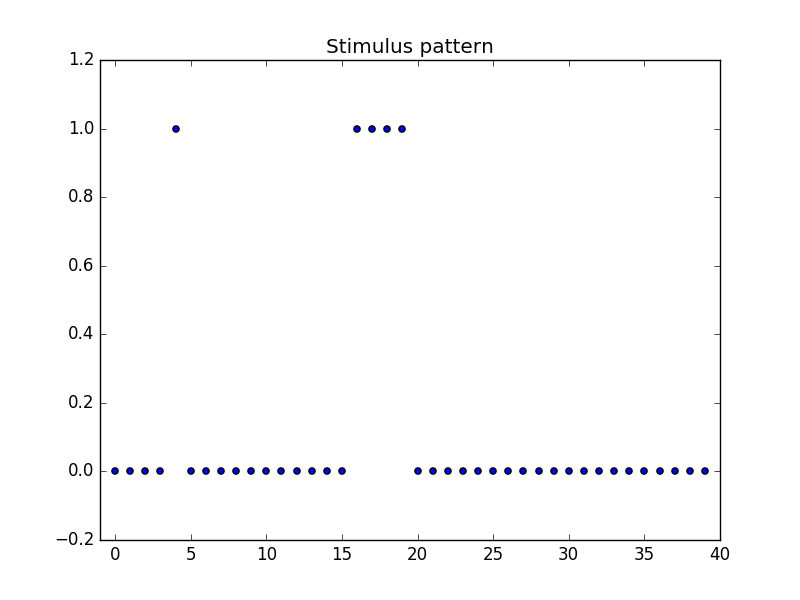
\includegraphics[width=.8\linewidth]{images/on_off_pattern.png} 
	\caption{$f$ (discrete stimulus)}
	\label{fig:on_off}
\end{minipage}	
\quad
\begin{minipage}[b]{0.45\linewidth}
	\centering
	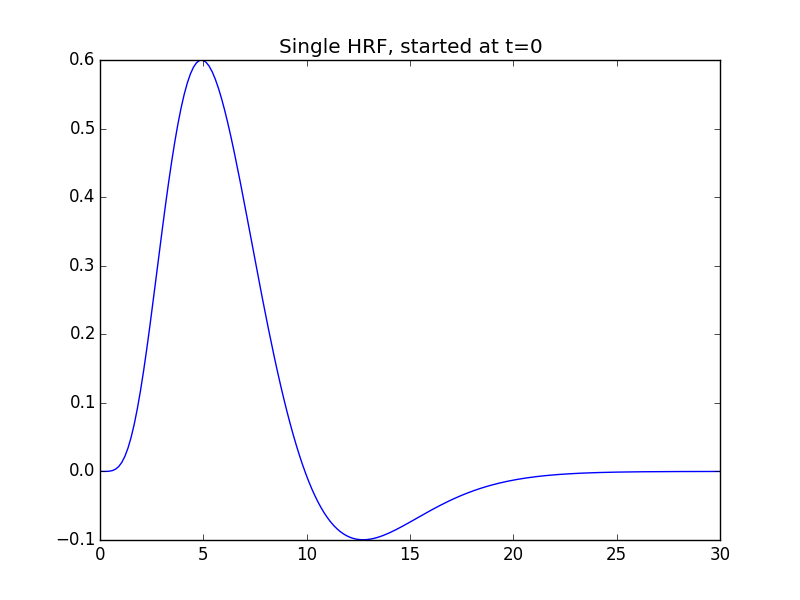
\includegraphics[width=.8\linewidth]{images/hrf_pattern.png} 
	\caption{$g$ (continous hrf)}
	\label{fig:hrf}
\end{minipage}
\end{figure}

With these examples of $f$ and $g$, we can convolve them to get what is 
seen in Figure \ref{fig:convolve1}.

\begin{figure}[ht]
	\centering
	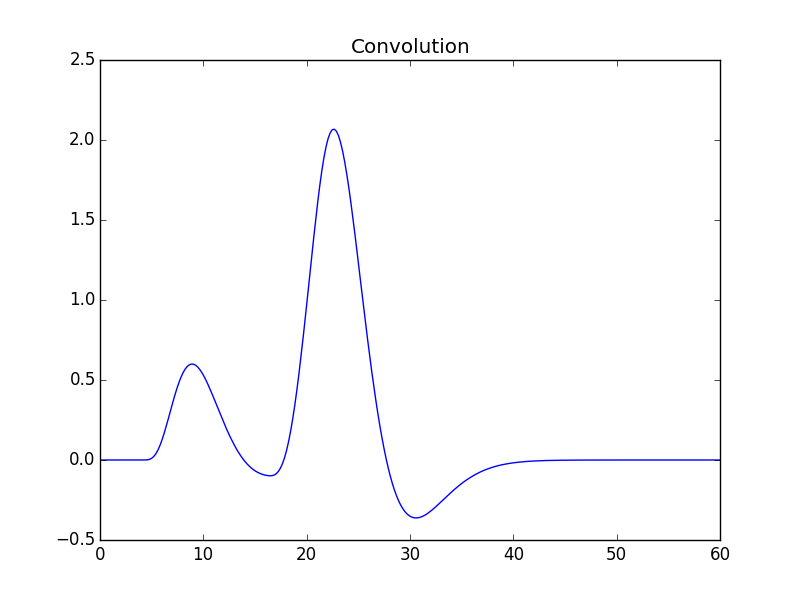
\includegraphics[width=.5\linewidth]{images/initial_convolved.png}
	\caption{convolution of $f$ and $g$}
	\label{fig:convolve1}
\end{figure}


Mathematically, convolution between $f$ and $g$ in can be described as:
\begin{equation}  \label{eq:standard_convolve}
r(t)= \sum_{i=1}^n \phi_{i}(t-t_i)
\end{equation}
where there are $i=1,...n$ stimuli points with a hemodynamic response for each 
being $\phi_i$, a function of $f(t_i)$ multiplied by the function $g(t)$.

In our case all the non-zero $f(t_i)$ are equal to 1, so all $\phi_i$ are the same. As such, we can rewrite this function as:
\begin{equation} \label{eq:generalized_hrf}
r(t) =\sum_{i=1}^n \phi (t-t_i)
\end{equation}

\section{Common Approach (\texttt{np.convolve})}

A common approach to convolve 2 functions in the way described above 
utilizes \texttt{np.convolve}, which uses fast fourier transforms for 
efficiency (it boils down to fewer computations using roots of unity). 
\texttt{np.convolve} assumes that the intervals between stimuli mirror the 
desired intervals between prediction intervals. It should be noted that 
\texttt{np} is a common notation for the \texttt{numpy} module in 
\texttt{python}.

\section{Moving beyond \texttt{np.convolve}, and needed improvements}

The reason motivating this appendix is that our data and needs fail to meet 
the assumption that the intervals are in equidistant. Especially in our case, 
there was not an easy route in terms of basic rounding to then correctly utilize 
\texttt{np.convolve}. All the following approaches improve on the basic 
\texttt{np.convolve} approach, but ultimately circle back to incorporating 
\texttt{np.convolve} for speed gains. 

\subsection{Our data/situation explained}
Our condition file (\texttt{cond1}) lists stimulus times for when the 
individual pumped the balloon but didn't pop it. For subject 001, the 
first 10 data points are as follows [Figure \ref{table:cond1}]:

\vspace{5mm}

\begin{figure}[ht]
\begin{center}
\begin{tabular}{|cccccccccc|}
  \hline
0.0671 &
2.1251 &
3.7681 &
5.6601 &
7.8673 &
9.3443 &
19.7831 &
22.0402 &
23.5837 &
25.1434 \\
 \hline

  \end{tabular}
   \caption{First 10 values for Sub 001, condition 1}
  \label{table:cond1}
\end{center}
\end{figure}
 
Clearly, this short time series doesn't align with scans that start at 
$t=0$ and occur every 2 seconds apart. As such, we had to go back to the 
drawing board to try to reproduce our expected hemodynamic reponse for the 
whole time course.



\subsection{Summary of Approaches}
Our first approach attempts to reproduce the theoretical rigor for our data. 
Our second approach tries to utilitize \texttt{np.convolve} by expanding the 
grid of desired results (thanks to advice from Jean-Baptiste Poline).




\subsubsection{Initial correction to represent theoretical idea}
To account for our data's lack of any easily identifiable grid structure 
between when a stimulus was recorded and when our scans occured (on the 
order of every 2 seconds), we went back to the theory of convolution and 
implemented code to recreate equation \ref{eq:standard_convolve} directly. 
To do so, we also had to create a function that treated all discrete points 
of $f$, the stimulus reponse as potential starts of the hemodyamic response, 
multiplied by the actual value of $f$, as see in equation 
\ref{eq:code_convolve}:

\begin{equation} \label{eq:code_convolve}
r(t)= \sum_{i=1}^n \psi_{i} \phi_{i}(t-t_i)
\end{equation}

where $psi_{i}$ is the value of $f$ at the $i$th element in the stimulus vector 
(allowing for zeroes and varying applitudes/strengths of stimulation).


\subsubsection{Matrix multiplication}
Equation \ref{eq:code_convolve}, rewritten below

$$r(t)= \sum_{i=1}^n \psi_i \phi_{i}(t-t_i)$$

can be changed to a matrix multiplication problem:

\begin{equation} \label{eq:matrix_code_convolve}
r(t)=  \psi \cdot \phi(t-t^*)
\end{equation}

where the $\phi$ is a vectorized function $t$ as a scalar output and $\psi$ is the vector of $f$ values (irrespective of location, as the $t^*$ takes that into account).


\subsubsection{Utilization of FFT with \texttt{np.convolve}}
The ''theoretical'' solution lacked computation efficiency (although the matrix version increased speed by a lot), so we also approached the problem by creating a more dense grid between each scan (2 seconds apart). Then we rounded the actual times of the stimulus to meet this more finely scaled grid. This allowed us to utilize \texttt{np.convolve} with it's faster algorithms (using FFT), and then reduce back down to our 2 second grid.

We initially started with 30 slices in between each scan, but matrix multiplication actually beat this analysis, so we reduced the time cost by 1/2 (with only 15 slices), and so little decline is accuracy.

This method does loose accuracy, but since the ideas behind this process don't really have very strong relationships to real life, a little accuracy loss is acceptable for speed.


%Needed references:
%Brett, Matthew and Poline, J-B  (2013). Convolution. Retrieved from http://practical-neuroimaging.github.io/on_convolution.html

\bibliography{project}

\end{document}
